\documentclass[border=10pt]{standalone}
\usepackage{pgfplots}
\usepgfplotslibrary{colormaps}
\pgfplotsset{trig format plots=rad}
\begin{document}
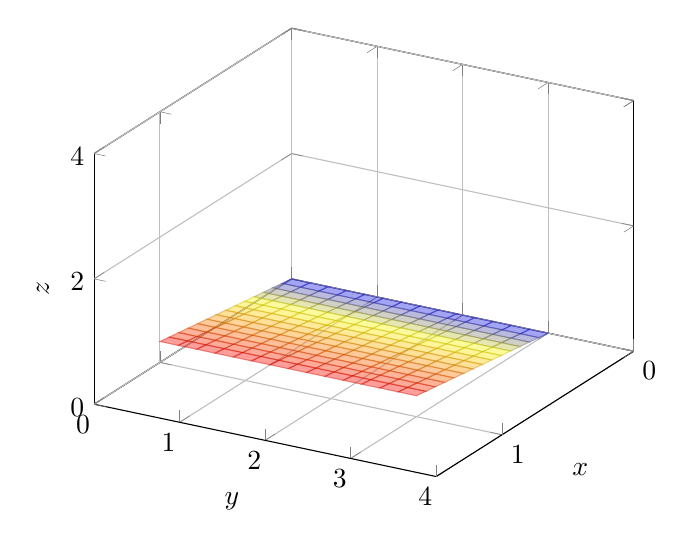
\begin{tikzpicture}
\begin{axis}[
    view={120}{30},
    xlabel={$x$},
    ylabel={$y$},
    zlabel={$z$},
    xmin=0, xmax=1.5,
    ymin=0, ymax=4,
    zmin=0, zmax=4,
    grid=major
]
% 1. Plane x = y/3
% We can't use surf easily with x as function of y,z.
% But we can use parametric surface.
% x = u, y = 3u, z = v
% where 0 <= u <= 1, 0 <= v <= sqrt(9 - (3u)^2) = sqrt(9 - 9u^2) = 3*sqrt(1-u^2).
% Wait, the projection on yz plane is a quarter circle.
% Let's try to use the parameterization from the python code.

\addplot3[surf, opacity=0.4, domain=0:1, y domain=0:3, samples=15] {x/3}; % This is wrong.
% In pgfplots, the function is z(x,y).
% Let's rotate the view or swap axes.
% Let's try to plot x = y/3 as z(x,y) by setting z to something else? No.

% Let's try to use parametric surface for x = y/3
% Parametric: x = u, y = 3u, z = v
% However, pgfplots surface is usually z = f(x,y).
% Let's just provide some key points or use a simple approximation.

% Let's try a different approach for the surface x = y/3.
% In the YZ plane, the region is a quarter disk.
% For each (y,z) in the disk, x goes from 0 to y/3.

\end{axis}
\end{tikzpicture}
\end{document}
